\documentclass{article}

\usepackage{graphicx}
\usepackage{tikz}
\usepackage{tikzsymbols}
\usetikzlibrary{calc,patterns,shapes.geometric}
\pagestyle{empty}
\usepackage[margin=0pt]{geometry}
\geometry{papersize={14in,12in}}

\def\centerarc[#1](#2)(#3:#4:#5){\draw[#1] ($(#2)+({#5*cos(#3)},{#5*sin(#3)})$) arc (#3:#4:#5);}

\begin{document}
	\begin{figure}
		\centering
		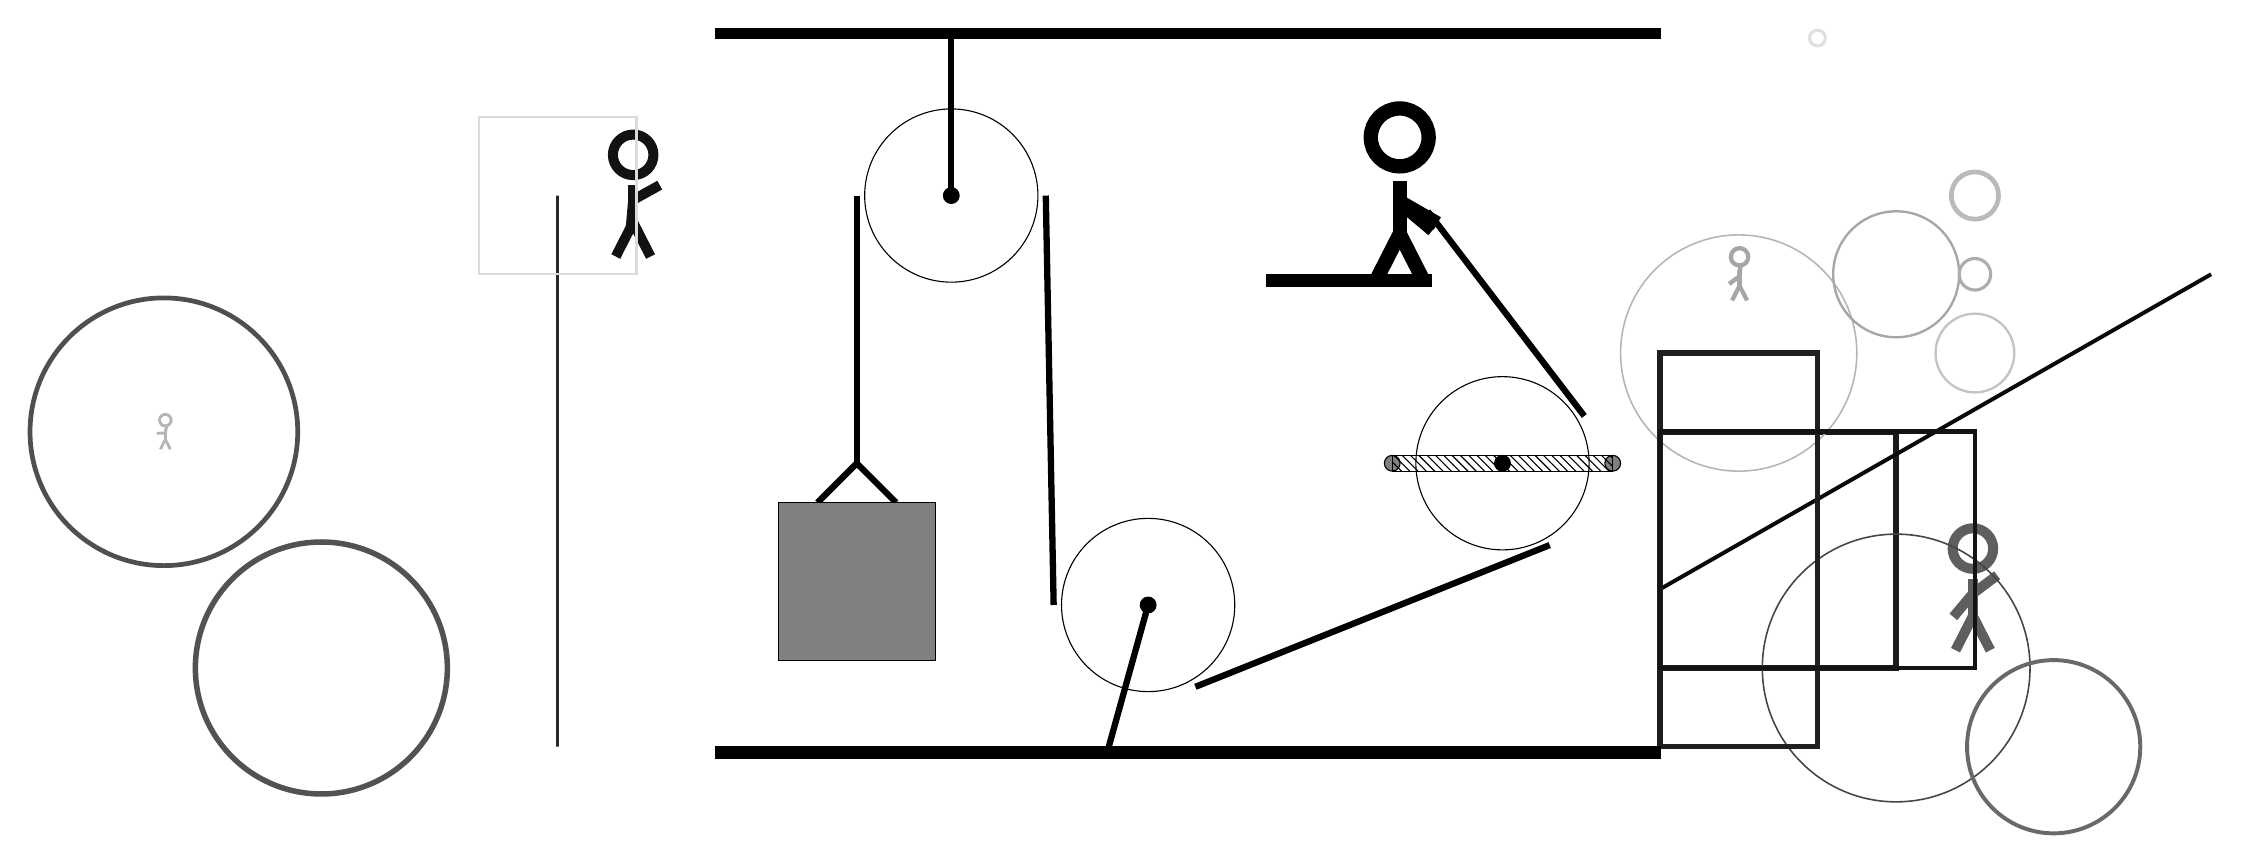
\begin{tikzpicture}
			%%%%% START %%%%%
			
			\draw[fill=black] (-2, 9) rectangle (10, 9.125);
			
			\node[line width=0.3mm, color=black!29] at (-9, 4) {\Strichmaxerl[2][2][79]};
			
			\draw [line width=0.7mm, color=black!15](-5, 3) circle (0.0);
			\draw[line width=0.7mm, color=black!89] (10, 1) rectangle (13, 4);
			\node[line width=0.7mm, color=black!63] at (14, 2) {\Strichmaxerl[7][50][37]};
			\node[line width=0.7mm, color=black!35] at (11, 6) {\Strichmaxerl[3][37][85]};
			
			\draw [line width=0.2mm, color=black!73](13, 1) circle (1.7);
			\draw[line width=0.4mm, color=black!84] (-4, 0) rectangle (-4, 7);
			\draw [line width=0.6mm, color=black!27](14, 7) circle (0.3);
			\draw [line width=0.7mm, color=black!68](-7, 1) circle (1.6);
			
			\draw [line width=0.5mm, color=black!59](15, 0) circle (1.1);
			
			\draw[line width=0.5mm, color=black!96](10, 2) -- (17, 6);
			\node[line width=0.6mm, color=black!93] at (-3, 7) {\Strichmaxerl[7][85][29]};
			\draw [line width=0.4mm, color=black!12](12, 9) circle (0.1);
			
			\draw [line width=0.3mm, color=black!23](14, 5) circle (0.5);
			\draw [line width=0.2mm, color=black!29](11, 5) circle (1.5);
			\draw[line width=0.3mm, color=black!14] (-3, 6) rectangle (-5, 8);
			
			\draw [line width=0.3mm, color=black!35](13, 6) circle (0.8);
			\draw[line width=0.7mm, color=black!88] (12, 5) rectangle (10, 0);
			\draw[line width=0.6mm, color=black!92] (10, 1) rectangle (14, 4);
			\draw [line width=0.4mm, color=black!32](14, 6) circle (0.2);
			\draw [line width=0.6mm, color=black!69](-9, 4) circle (1.7);
			
			
			\draw (1, 7) circle (1.1);
			\draw[fill=black] (1, 7) circle (0.1);
			\draw[line width=0.8mm] (1, 9) -- (1, 7);
			
			\draw (3.5, 1.8) circle (1.1);
			\draw[fill=black] (3.5, 1.8) circle (0.1);
			\draw[line width=0.8mm] (3.5, 1.8) -- (3.0, 0);
			
			\draw[fill=white](8, 3.6) circle (1.1);
			\draw[fill=black] (8, 3.6) circle (0.1);
			\draw[fill=black!50] (9.4, 3.6) circle (0.1);
			\draw[fill=black!50] (6.6, 3.6) circle (0.1);
			\draw[pattern=north west lines, pattern color=black] (6.6, 3.7) rectangle (9.4, 3.5);
			
			\draw[line width=0.8mm](-0.7, 3.1) --  (-0.2, 3.6) -- (0.3, 3.1);
			\draw[fill=black!50] (-1.2, 3.1) rectangle (0.8, 1.1);
			
			\draw[line width=0.8mm](-0.2, 7) -- (-0.2, 3.6);
			\centerarc[line width=0.8mm](1, 7)(180:0:1.2000000000000002)
			\draw[line width=0.8mm](2.2, 7) -- (2.3, 1.8);
			\centerarc[line width=0.8mm](3.5, 1.8)(180:300:1.2000000000000002);
			\draw[line width=0.8mm](4.1, 0.7608) -- (8.6, 2.5608);
			\centerarc[line width=0.8mm](8, 3.6)(300:390:1.2000000000000002);
			\draw[line width=0.8mm](9.0392, 4.2) -- (7.05, 6.8);
			
			\node at (6.75, 7) {\Strichmaxerl[10][-220][-30]};
			\draw[fill=black] (5, 6) rectangle (7.1, 5.85);
			
			\draw[fill=black] (-2, 0) rectangle (10, -0.15);
			
			%%%%% END %%%%%
		\end{tikzpicture}
	\end{figure}	
\end{document}